\documentclass{article}

% to give various notational syntax
\usepackage{amsmath,amsthm,amssymb, mathtools, enumerate, physics}

% for including images
\usepackage{graphicx}
\graphicspath{ {../../Images/} }
% Resize figures that are too wide for the page.
\makeatletter
\def\ScaleIfNeeded{%
  \ifdim\Gin@nat@width>\linewidth
    \linewidth
  \else
    \Gin@nat@width
  \fi
}
\makeatother
\let\oldincludegraphics\includegraphics
\renewcommand\includegraphics[2][]{%
  \oldincludegraphics[width=\ScaleIfNeeded]{#2}
}
%
%% for bibliography and citation
%\usepackage[square,compress]{natbib}
%\setcitestyle{super,comma}
%\bibliographystyle{unsrtnat}
%
%% for executing and including python code
%\usepackage{pythontex}
%
%% for defining lovely colors
%\usepackage{xcolor}
%\definecolor{light-gray}{gray}{0.95}
%
%% for syntax highlighting of non-python languages
%\usepackage{minted}
%\usemintedstyle[cpp]{manni}
%\newcommand{\cpp}[1]{\mintinline{cpp}{#1}}

% for linking sections of the document and table of contents
\usepackage{hyperref}
\hypersetup{
    colorlinks=true, %set true if you want colored links
    linktoc=all,     %set to all if you want both sections and subsections linked
    linkcolor=blue,  %choose some color if you want links to stand out
}


\newcommand{\nn}{\newline\newline}
\newcommand{\n}{\newline}
\newcommand{\bq}{\begin{equation}}
\newcommand{\eq}{\end{equation}}
\newcommand{\ba}{\begin{align}}
\newcommand{\ea}{\end{align}}
\newcommand{\bi}{\begin{itemize}}
\newcommand{\ei}{\end{itemize}}
\newcommand{\ct}[1]{\citep{#1}}

\newcommand*{\Perm}[2]{{}^{#1}\!P_{#2}}
\newcommand*{\Comb}[2]{{}^{#1}C_{#2}}




\begin{document}

\title{Conditional Probability}
\date{}
\maketitle

\noindent
\textbf{Question}: What is the definition of a conditional probability?
\nn
\textbf{Question}: What is the definition of disjoint and the definition of independent?
\nn
\textbf{Question}: What is the general Multiplication Rule (the probability of an intersection of sets)?
\nn
\textbf{Question}: Derive the Law of Total Probability (the probability of an event by partitioning) and Bayes Formula (the conditional probability without knowing the prior i.e. denominator of Bayes rule).
\nn
\textbf{False Positive Problem}: Calculate the probability that a random person who has tested positive for the disease actually has it. The frequency of the disease in the population is 0.01, the rate of false positives is 0.01 and false negatives is 0.001. \textbf{Hint: Draw a picture!}
\nn
\textbf{Frog Problem:} A frog starts on a lily pad and takes his first hop to wind up on one of three lily pads $\{A_1,A_2,A_3\}$. He takes his second hop to wind up on one of three other lily pads $\{B_1,B_2,B_3\}$. We know the transition probabilities for these hops. After his journey I observe the frog at pad $B_2$. What is the probability that he arrived via pad $A_1$? Before he starts over for his next journey I would like to know the probability he will end up on pad $B_1$.\n

\vspace{.3 in}

\tableofcontents

\section{Conditional Probability \& False Positives}
The conditional probability of B given A, $P(A|B)$ is the probability that event B has occurred given that A has definitely occurred. It is easy to derive an expression for conditional probability by visualizing surface area as a probability measure over a 2-d region.
\nn
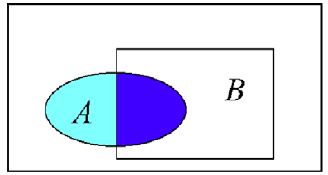
\includegraphics{conditional} 

Knowing that A occurs collapses our universe into the oval, which we can think of as our new sample space with a probability of one. The probability that B occurs is then the ratio of the area in which B holds in our new universe to the total area of our new sample space (which is now the oval). 
\begin{equation}
P(B|A) = \frac{P(A\cap B)}{P(A)}
\end{equation}
\n




\section{Disjoint vs. Independent Events}

Two events (sets) are \textbf{disjoint} if they share no elements, $A\cup B = \emptyset$. In the area geometric picture they are non-overlapping regions. For two disjoint events we  get a nice sum rule that $P(A\cup B)=P(A)+P(B)$.
\nn

Two events (sets) are \textbf{independent} if being given information about the occurrence of one of them does not give information about the occurence of the other. In terms of conditional probability, \textbf{A and B are independent iff $P(B|A) = P(B)$}. In this case it's easy to show that we also have $P(A|B) = P(A)$. In terms of the the area measure picture, independence means that the proportion of A that B overlaps is the same as the proportion of the sample space that B occupies - the \textit{fraction} of area where B holds true does not change when our universe is collapsed to A, that is why we don't gain any information about the occurence of B.
\n\n

\subsection{Multiplication Rule}
Note that for independent events we get a simplified \textbf{Multiplication Rule} that $P(A\cap B)=P(A)P(B)$, where in general from the conditional probability expression we have $P(A\cap B)=P(A)P(B|A)$. This can be applied iteratively to get an expression for any arbitrary intersection,
\begin{equation}
\mathrm  P\left(\bigcap_{k=1}^n A_k\right)  = \prod_{k=1}^n  \mathrm P\left(A_k \,\Bigg|\, \bigcap_{j=1}^{k-1} A_j\right)
\end{equation}
\nn

Note that if two events are disjoint then they are certainly dependent since if I know that A has occurred then I know for sure that B has definitely NOT occurred. Also note that although the intuitive interpretation of two events being independent is that they are not causally related, it is possible for this not to be the case. It could be a matter of luck that the ratios of areas discussed above work out to be the same.


\section{Law of Total Probability \& Bayes Formula}

The law of total probability helps you find the total probability of an event by considering the different mutually exclusive ways it could happen. \textbf{Partitioning} a sample space means to break it into a set of disjoint events, $\{A_i\}$ (the mutually exclusive areas), whose union is the full sample space $S$. The total probability for any event $B$ in $S$ must be:
\begin{align}
P(B) = \sum_iP(A_i\cap B) \textrm{ which holds because the partitions are disjoint.}\\
= \sum_iP(A_i)*P(B|A_i), \textrm{ using the conditional probability formula.}
\end{align}

Bayes formula makes use of this expression for $P(B)$ to consider the probability of being in a specific partition $A_i$, given that you are in $B$. We expect this to be the portion of $B$ that is taken up by overlap with $A_i$.
\begin{align}
P(A_i|B) = \frac{P(A_i\cap B}{P(B)} = \frac{P(A_i\cap B}{\sum_jP(A_j)*P(B|A_j)} \textrm{ using total probability.}\\
= \frac{P(A_i)*P(B|A_i)}{\sum_jP(A_j)*P(B|A_j)}.
\end{align}


\section{False Positive Problem}
If A is the event that the random person chosen from our population has the disease and B is the event that the person has a positive test result, then we want $P(A|B) = \frac{P(A\cap B)}{P(B)}$. 
\n
We can interpret the provided information as:
\begin{align}
P(\bar{B}|A) = \text{false negative rate} = 0.001\\
P(B|\bar{A}) = \text{false positive rate} = 0.01\\
P(A) = \text{incidence in general population} = 0.01 \implies P(\bar{A}) = 0.99
\end{align}
Using Bayes formula again to recast the numerator, and using partitioning a la the Law of Total Probability to recast the denominator, 
\begin{equation}
P(A|B) = \frac{P(A\cap B)}{P(B)} = \frac{P(B|A)P(A))}{P(A)P(B|A)+P(\bar{A})P(B|\bar{A})}
\end{equation}
It remains to find $P(B|A)$, the probability of testing positive given that the person has the disease. We can again use partitioning since the event of having the disease is split between correct positives (the probability we are interested in) and false negatives, that is
\begin{equation}
1 = P(B|A) + P(\bar{B}|A) \implies P(B|A) = 0.999
\end{equation}
So we have finally
\begin{equation}
P(A|B) = \frac{(0.999)(0.01)}{(0.01)(0.999)+(0.99)(0.01)} = 4.7\%
\end{equation} 
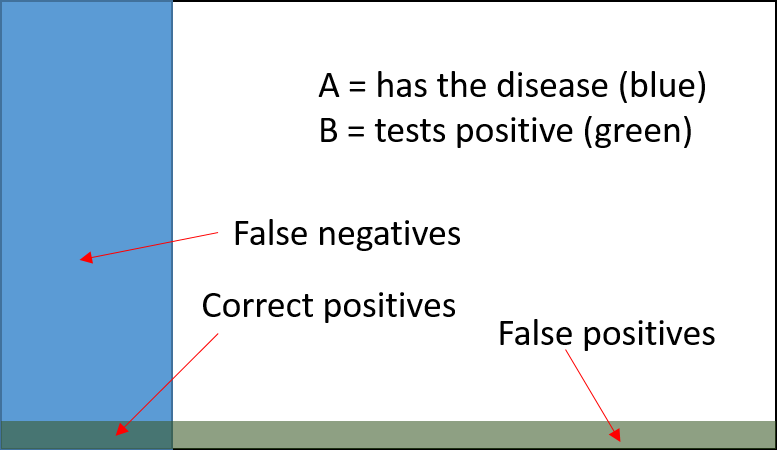
\includegraphics{falsepositive}
\n

\section{Frog Problem}
Consider a sample space where each element is a path that the frog took. We observe him to end up on $B_2$ so our universe collapses to the set of paths that ended on $B_2$. Within our new universe we want to know the probability he went via pad $A_1$ - this is the probability $P(A_1|B_2)=\frac{P(A_1\cap B_2)}{P(B_2)}$. The transition probabilities we know for the first hop correspond to the $P(A_i)$ while the transitions we know for the second hop correspond to the $P(B_j|A_i)$, so we need to recast the previous expression in terms of these quantities. First note $P(A_1\cap B_2)=P(B_2\cap A_1)=P(B_2|A_1)P(A_1)$ - both of which we have. We also can use the partitioning, or the law of total probability to say $P(B_2) =\sum_i P(B_2|A_i)P(A_i)$ - which answers the second question as well. 

\end{document}